
\documentclass[12pt]{article}
\pagestyle{empty}
\setlength{\parskip}{0in}
\setlength{\textwidth}{6.8in}
\setlength{\topmargin}{-.5in}
\setlength{\textheight}{9.3in}
\setlength{\parindent}{0in}
\setlength{\oddsidemargin}{-.7cm}
\setlength{\evensidemargin}{-.7cm}

\usepackage{amsmath}
\usepackage{amsthm}
\usepackage{amstext}

\usepackage{graphicx}

\begin{document}

{\bf MAT 105 Final Exam (white) Fall 2009} \hspace{.4in} {\large Name} \hrulefill

\hspace{.2in}

\begin{center}

\begin{tabular}
{|l|c|c|c|c|c|c|c|c|c|c|c|c|c|c|c|c|} \hline

 Problems & \hspace{5 pt} 1 \hspace{5 pt}  & \hspace{5 pt} 2 \hspace{5 pt} & \hspace{5 pt} 3 \hspace{5 pt} & \hspace{5 pt} 4 \hspace{5 pt}& \hspace{5 pt} 5 \hspace{5 pt} & \hspace{5 pt} 6 \hspace{5 pt} & \hspace{5 pt} 7 \hspace{5 pt}   & \hspace{5 pt} 8 \hspace{5 pt} &  \hspace{5 pt} Total  \hspace{5 pt} & &  \hspace{5 pt} Grade \hspace{5 pt}  \\ \hline
&&&&&&&&&&&\\  
Points &&&&&&&&&&   \hspace{.6in}\% &  \\ 
&&&&&&&&&&& \\  \hline
Out of & 40  & 14 & 28 & 22 & 38 & 17 & 22 & 19 &200 & & \\ \hline

\end {tabular}
 
\end{center}

\hspace{.2in}

\begin{itemize}
\item Relax.  You have done problems like these before. Even if these problems look a bit different, just do what you can. 
\item  If you're not sure of something or if you're stuck, please ask! 
\item You may use your calculator but please show all of your work and write down as many steps as you can.  
\item Some formulas from our book that you might need are on a separate sheet.
\item Don't spend too much time on any one problem.
\item  Do well.  And remember to ask me if you need help.
\end{itemize}

  \vspace{.2in}
 
 \hrulefill
 
\newpage  %%%

\begin{enumerate}
\item Evaluate each of the following expressions.

\begin{enumerate}
\item $59.99 - 0.79(30)=$
\vfill
\item $(12)^2-4(-9.8)(2)=$
\vfill
\item $500(1.06)^{36}=$
\vfill
\item $\displaystyle \frac{-(27)}{2(-16)}=$
\vfill
\item $3^{45}=$
\vfill
\item $(7.3)^{1/10}=$
\vfill
\item $\sqrt{267}=$
\vfill
\item $\displaystyle \frac{\text{log}(34.66)}{\text{log}(1.13)}=$
\vfill
\emph{Write the next answer in normal (expanded) decimal notation.}
\item $2.89 \times 10^{15}=$  


\vfill
\emph{Write the next answer in normal (expanded) decimal notation.}
\item $2.89 \times 10^{-15}=$  


\vfill
\end{enumerate}

\newpage  %%%

\item The 1918 flu season was one of the deadliest in history.  The graph and table show the number of flu deaths in Manchester, United Kingdom during 1918.

\begin{center}
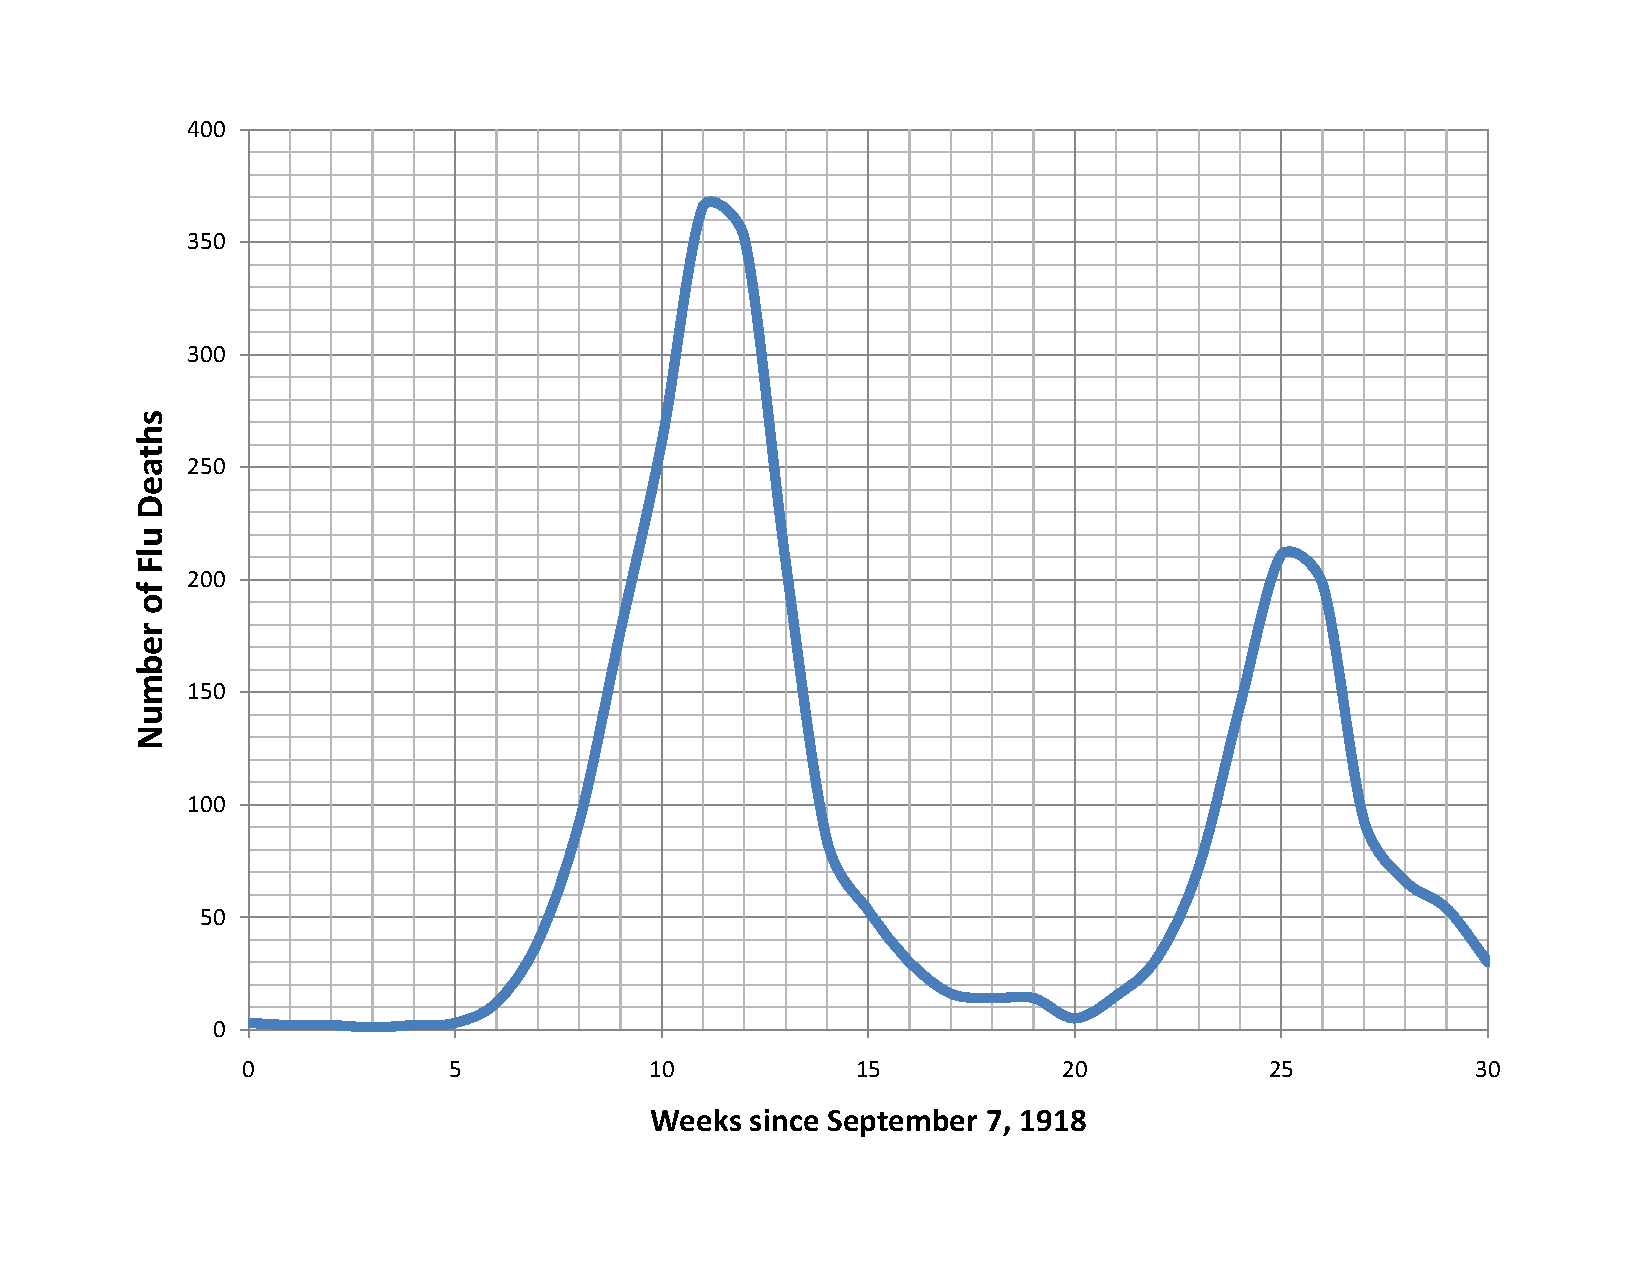
\includegraphics [width = .8\textwidth] {ManchesterFlu.pdf}
\end{center}

\begin{tabular} {|c|c|c|c|c |c|c|c|c|c |c|c|} \hline
Weeks since Sept. 7, 1918 & 0 & 3 & 6  & 9  & 12  & 15  & 18 & 21  & 24  & 27  & 30 \\ \hline
Number of deaths &3 & 1 & 12 & 177 & 352 & 53 & 14 & 15 & 14 & 93 & 30 \\ \hline
\end{tabular}

\begin{enumerate}
\item How many people died from the flu 9 weeks after September 7?
\vfill
\item In what weeks after September 7 did the number of flu deaths drop back to the level at 9 weeks?
\vfill
\item In what week after September 7 was the number of flu deaths the highest and what were the approximate number of deaths?
\vfill
\item Was the number of weekly flu deaths increasing faster 9 weeks after September 7 or 21 weeks after September 7?  Explain. (\emph{Hint: Determine the average rate of change at both of these times.})
\vfill
\end{enumerate}

\newpage %%%

\item My plumber charges $P$ dollars for $H$ hours of work, as given by the following formula:
$$P = 24.95 + 85.00H$$

\begin{enumerate}
\item Make a table of values showing the charges for 1 hour, 1$\frac{1}{2}$ hours, 2 hours, and 3 hours.
\vfill
\item What does the 24.95 represent and what are its units?
\vfill
\item What does the 85.00 represent and what are its units?
\vfill
\item If the bill for my plumber's last visit was $\$218.75$, how much time did she work?

\emph{Set up and solve an equation to answer the question.  If you can't solve it, then you may estimate the answer to two decimal places for possible partial credit.}
\vfill
\vfill
\vfill
\item Convert your answer to the nearest minute.
\vfill
She worked for \hrulefill hours, \hrulefill minutes. \hspace{3in}.
\end{enumerate}
\pagebreak
\item The timing of the sunset depends on the latitude (how far North of South of the equator one is) and the time of year.  In Minneapolis, the sunset occurred at 6:01 PM on March 1.  The time of the sunset is expected to occur 1.26 minutes later each day.  In Galveston, Texas, the sunset occurred at 6:19 PM on March 1 and is expected to occur 0.58 minutes later each day.  (Note: do not worry about Daylight Savings Time.) If we let $S$ represent the time of the sunset (in minutes since 6 PM) for $D$ days after March 1, then the equations are:

\vspace{.1in}

\begin{center}
\begin{tabular} {ll} 
Minneapolis: &$S=1+1.26D$ \\
Galveston: & $S=19+0.58D$ \\
\end{tabular}
\end{center}

The table shows sunset times for the two cities:

\begin{center}
\begin{tabular} {|l|r|r|r|r|} \hline
$D$ & 0 & 5 & 15 & 31 \\ \hline
$S$ (Minneapolis) & 1 &  7.3 & 19.9 & 40.1  \\ \hline
$S$ (Galveston) & 19 & 21.9 & 27.7 & 37.0 \\ \hline
\end{tabular}
\end{center}

\begin{enumerate}

\item Which city has a later sunset on March 10 (i.e. after 10 days)?  \emph{Justify your answer.}
\vfill

\item Draw a graph illustrating both equations.
\vspace{.1in}
\begin{center}
\scalebox {.8} {
\includegraphics [width = 6in] {../GraphPaper}}
\end{center}
\vfill
\emph{The problem continues on the next page ...}
\pagebreak
\item Set up and solve an equation to find when the two cities will have the sunset at the same time. Report your answer to the nearest day.

\emph{Just approximating the answer will get almost no partial credit.}

\vfill
\vfill
\vfill
\end{enumerate}

\newpage %%%

\item A diver jumps up in the air from a 7.5-meter board.  His height above the water, $H$ meters, after $T$ seconds is given by the formula: $$H = 7.5 + 3.1T - 4.88T^2$$

\begin{enumerate}
\item Complete the following table of values.

\emph{Please report your answers to two decimal places.}

\begin{center}
\begin{tabular} {|l|c|c|c|c|c|c|} \hline
$T$ & 0 & 0.5 & 0.8 & 1.0 & 1.4 & 1.8 \\ \hline
&&&&&& \\
$H$ & \hspace{.7in} & \hspace{.7in}  & \hspace{.7in}  & \hspace{.7in}  & \hspace{.7in}  & \hspace{.7in}  \\
&&&&&& \\ \hline
\end{tabular}
\end{center}

\item How high up in the air does the diver get?

\emph{Find the answer to two decimal places using whatever method you prefer.}
\vfill
\vfill

\item Convert your answer to the nearest foot.  \emph{Use 1 meter = 3.28 feet.}
\vfill

\hspace{-.5in} \emph{The problem continues on the next page.}

\newpage %%%

\item Draw a graph illustrating the dependence.

\vspace{.1in}
\begin{center}
\scalebox {.8} {
\includegraphics [width = 6in] {../GraphPaper}}
\end{center}
\vspace{.1in}

\item When does the diver hit the water?

\emph{Find the answer to two decimal places using whatever method you prefer.}

\vfill
\end{enumerate}

\newpage %%%
%%% http://www.energywatchgroup.org/fileadmin/global/pdf/2009-01_Wind_Power_Report.pdf

\item A recent summit in Copenhagen is focusing on climate change and its impacts.  Increasing carbon dioxide emissions are a cause of concern because of their linkages to climate change.  In 1959 (when modern instruments could first measure carbon dioxide concentrations), the average concentration in the Northern Hemisphere was 316 parts per million (ppm) CO$_{2}$.  That is to say, there were 316 CO$_{2}$ molecules for every million molecules of air.  In 2008, the concentration of CO$_{2}$ was 386 ppm CO$_{2}$.  Assuming this increase is exponential, from 1959 to 2008 the CO$_{2}$ concentration grew at a rate of 0.41\% per year.  That is, the CO$_{2}$ concentration $C$ (in ppm) $Y$ years after 1959 is given by the equation:

$$C=316(1.0041)^Y$$

\begin{enumerate}
\item According to this equation, what will the CO$_{2}$ concentration be in 2010?
\vfill
\item If the value continues to increase, in what year will the CO$_{2}$ concentration be over 400 parts per million CO$_{2}$?

\emph{Set up and solve an equation to answer the question.  If you can't solve it, then you may estimate the answer for possible partial credit.}
\vfill
\vfill
\vfill
\end{enumerate}

\newpage %%%

\item When I moved to my new house I had to rent a UHaul to move all my stuff.  The table below lists the rental charges for the truck.  UHaul charges an initial fee plus an hourly rate.

\begin{center}
\begin{tabular} {|r|r|r|r|r|r|r|} \hline
Hours & 1 & 2 & 3 & 4 & 5 & 10 \\ \hline
Cost & \$19.95 & \$26.80 & \$33.65 & \$40.50 & \$47.35 & \$81.60 \\ \hline
\end{tabular}
\end{center}

\begin{enumerate}
\item Name the variables including units.
\vfill
\item What does UHaul charge per hour to use the truck?
\vfill
\item What is the initial fee?
\vfill
\item Write an equation describing the cost of renting a truck.
\vfill
\end{enumerate}

\newpage %%%

\item I was boiling water on the stove for some tea.  When I took it off the stove it was boiling at a temperature of 212 degrees Fahrenheit. The tea was cool enough to drink at a temperature of 100 degrees Fahrenheit 20 minutes later. You can assume that the coffee cools exponentially.

\begin{enumerate}
\item By what percentage does the coffee temperature decrease each minute?
\vfill
\item What will the coffee temperature be 10 minutes later (i.e.\ after 30 minutes total)?
\vfill
\end{enumerate}



\end{enumerate}

\end{document}

